\section{TRABALHOS RELACIONADOS}
\label{sec:trabalhos-relacionados}
\citeonline{utfpr2017} propõe em seu trabalho a produção de um recurso educacional para auxiliar o ensino de análise e projeto de \textit{software}. Para suprir a necessidade da prática em matérias de ES, principalmente para os cursos de Engenharia Elétrica, de Computação e Controle e Automação. O recurso educacional proposto consiste em um conjunto de projetos utilizando a plataforma Arduino. Cada projeto possui seis artefatos: o diagrama de casos de uso, o diagrama de atividades, o diagrama de maquinas de estado, o diagrama de classe, o esquemático de montagem e o código fonte em linguagem C/C++. A partir destes artefatos os alunos deveriam analisá-los e embarcá-los na plataforma Arduino, de forma a treinar a capacidade de interpretação de artefatos UML. Os artefatos foram aplicados em 3 turmas do curso de Engenharia de Computação da UTFPR - Câmpus Cornélio Procópio, durante a disciplina de Engenharia de \textit{Software}, onde após a conclusão da utilização, os alunos deram um \textit{feedback} através de um questionário baseado na escala \textit{likert} e uma questão aberta, para possíveis sugestões. As respostas a respeito do recurso educacional foram predominantemente positivas, demonstrando a aceitação pelos alunos e o auxílio no aprendizado.

\citeonline{Garcia2017} apresenta o GOAL (Gamification on Application Lifecycle Management), um \textit{framework} que tem como objetivo a orientação de um processo que suporta a introdução da gamificação em qualquer fase do desenvolvimento de \textit{software}. Um estudo de caso foi realizado pelos autores em uma empresa de desenvolvimento de \textit{software} para investigar a viabilidade de aplicação do \textit{framework} para integrar a gamificação em outros ambientes de engenharia de \textit{software}. Foram gamificadas três áreas de processo utilizando uma metodologia presente no GOAL, as áreas são: gerenciamento de requisitos, gerenciamento de projetos e teste de \textit{software}. Os elementos de jogos escolhidos para a gamificação foram: pontuação, \textit{levels}, distintivos, \textit{leaderboard}, \textit{social graph} e desafios. As conclusões obtidas em relação a utilização do \textit{framework} foram positivas, revelando benefícios oferecidos na utilização do GOAL em um contexto industrial. 

\chapter{PROPOSTA}
\label{chap:proposta}

Nesta seção são descritas as atividades que serão executadas a fim de atingir os objetivos deste trabalho, bem como as tecnologias utilizadas para o desenvolvimento do mesmo. Esta seção está subdivida em: plicação, ferramentas e utilização da aplicação e \textit{feedback} análise dos resultados.  

\section{APLICAÇÃO WEB}
\label{sec:desenvApp}



O artefato produzido por este trabalho será uma aplicação web, composta por uma breve introdução sobre a plataforma Arduino e um pequeno projeto a ser desenvolvido, para ambientar os usuários ao cenário. Após isso, será apresentado três áreas de conhecimentos abordadas no projeto, como apresentado na Figura \ref{fig:figura-areas-telas}, onde cada uma será constituída por uma introdução, questionário sobre conceitos e atividades práticas divididas em fases, como visto na Figura \ref{fig:figura-fases-telas}. O avanço em cada fase se dará somente após a resolução do exercício proposto e submissão para correção. A cada fase, o nível de complexidade do projeto será aumentado gradativamente.

\begin{figure}[!htb]
    \centering
    \caption{Áreas de conhecimento}
    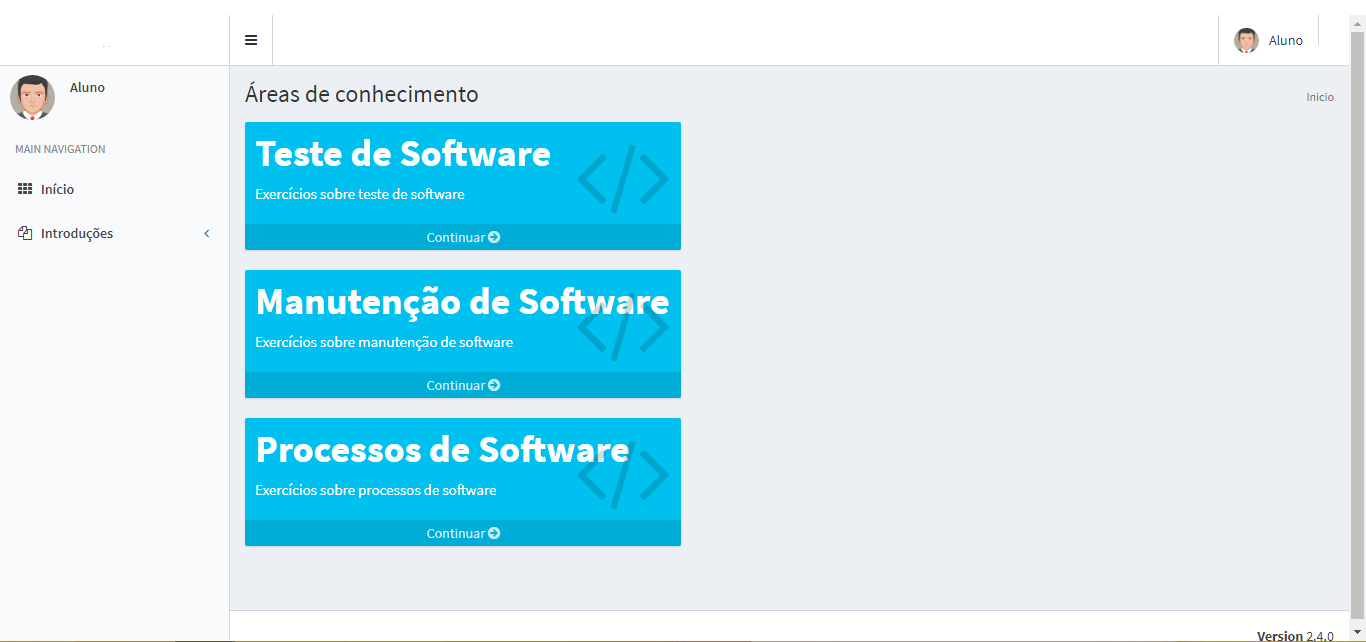
\includegraphics[width=1\textwidth]{./dados/figuras/areasTela}
    \fonte{Autoria Própria}
    \label{fig:figura-areas-telas}
\end{figure}

\begin{figure}[!htb]
    \centering
    \caption{Fases sobre teste de \textit{software}}
    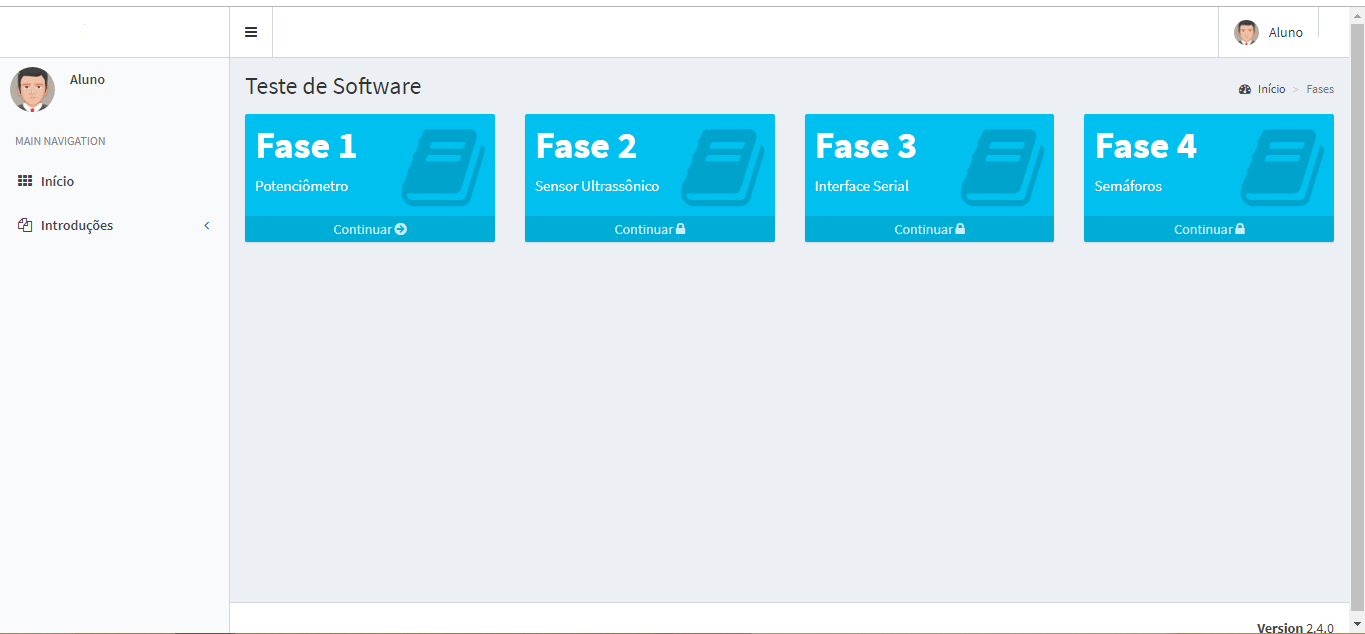
\includegraphics[width=1\textwidth]{./dados/figuras/fasesTela}
    \fonte{Autoria Própria}
    \label{fig:figura-fases-telas}
\end{figure}
 
Em cada fase será apresentado qual o objetivo, uma breve descrição, quais itens e componentes serão necessários, uma imagem do esquemático do projeto para montagem do circuito e um \textit{sketch}. Com essas informações o aluno deverá reconstruir o cenário proposto e realizar a atividade, que poderá surtir efeitos no \textit{sketch}, esquemático, diagramas de classe dos itens utilizados, diagramas de casos de uso, diagramas de atividade ou diagramas de máquina de estado do projeto. A Figura \ref{fig:figura-fase-tela} ilustra um exemplo de tela de uma das fases. Nela, o aluno realiza a leitura das atividades e tem acesso ao \textit{sketch}, esquemático e diagramas, para o auxílio na montagem do projeto. 
\begin{figure}[!htb]
    \centering
    \caption{Fase 1 - teste de \textit{software}}
    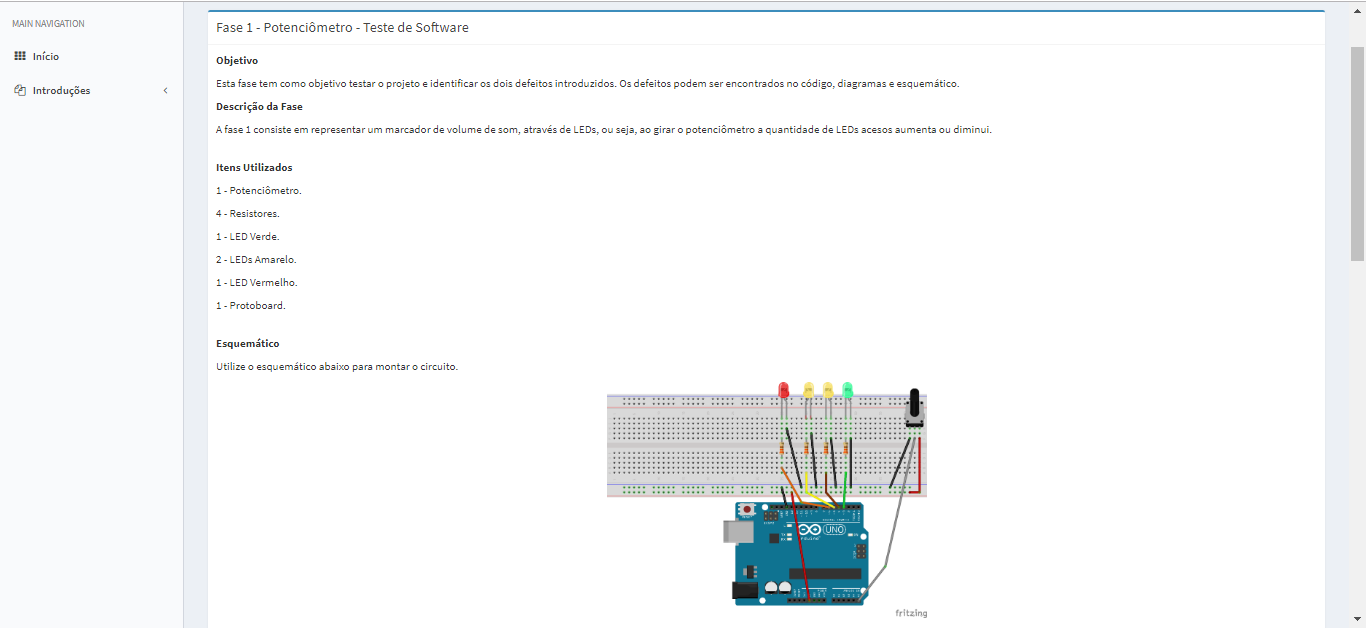
\includegraphics[width=1\textwidth]{./dados/figuras/faseTela}
    \fonte{Autoria Própria}
    \label{fig:figura-fase-tela}
\end{figure}

\section{FERRAMENTAS}
\label{sec:ferramentas}

\section{EXECUÇÃO DA APLICAÇÃO E ANÁLISE DE RESULTADOS}
\label{sec:execAppAnaliseResultados}
Para a avaliação da aceitação, motivação, engajamento, consolidação e aquisição de conhecimento causado pelo artefato gerado neste trabalho, o mesmo será utilizado por alunos da disciplina Engenharia de \textit{Software}, que possuem um conhecimento prévio sobre linguagem de programação, orientação a objetos, circuitos eletrônicos e alguns conceitos nos temas abordados neste trabalho. Ao término da utilização, os alunos darão um \textit{feedback} através de um questionário baseado na escala \texttt{likert}, um tipo de escala psicométrica comumente utilizada em pesquisas de opinião, onde a cada afirmação o pesquisado deve escolher um valor de 1 a 5. O valor um retrata o total desacordo ou negação, e o valor cinco representa o total acordo ou aceitação.


\chapter{CRONOGRAMA}
\label{chap:cronograma}